\documentclass[11pt,a4paper]{article}

% --- Paquetes de Estilo y Formato ---
\usepackage[utf8]{inputenc}
\usepackage[spanish,es-tabla]{babel}
\usepackage[T1]{fontenc}
\usepackage{geometry}
\geometry{top=3cm, bottom=3cm, left=3cm, right=2.5cm}
\usepackage{tabularx}
\usepackage{titlesec}
\usepackage{fancyhdr}
\usepackage{lastpage}
\usepackage{hyperref}
\usepackage{enumitem}
\usepackage{graphicx}
\usepackage{tikz}
\usepackage{float}
\usepackage{array}
\usepackage{colortbl}
\usepackage[table, xcdraw]{xcolor}

% --- Definición de Colores Corporativos ArthroDesign ---
\definecolor{ArthroNavy}{HTML}{0F172A}
\definecolor{ArthroTeal}{HTML}{0D9488}
\definecolor{ArthroGray}{HTML}{64748B}
\definecolor{tabblue}{RGB}{173, 204, 230}

% --- Configuración de Párrafo ---
\setlength{\parskip}{0.5em}
\setlength{\parindent}{1.5em}

% --- Estilo de Títulos con Identidad Corporativa ---
\titleformat{\section}
  {\color{ArthroNavy}\Large\bfseries}
  {\thesection.}
  {0.5em}
  {}
  [{\color{ArthroTeal}\titlerule[1.5pt]}]

\titleformat{\subsection}
  {\color{ArthroNavy}\large\bfseries}
  {\thesubsection.}
  {0.5em}
  {}
  [{\color{ArthroTeal}\titlerule[1pt]}]

\titleformat{\subsubsection}
  {\color{ArthroNavy}\large\bfseries}
  {\thesubsubsection.}
  {0.5em}
  {}

% --- Viñetas en color Turquesa ---
\renewcommand{\labelitemi}{\color{ArthroTeal}\textbullet}
\renewcommand{\labelitemii}{\color{ArthroTeal}\circ}

% --- Configuración de Enlaces ---
\hypersetup{colorlinks=true, linkcolor=ArthroNavy, urlcolor=ArthroTeal}

% --- CONFIGURACIÓN DE ENCABEZADO Y PIE CORPORATIVO (Anexo I) ---
\pagestyle{fancy}
\fancyhf{}

% Línea superior de color turquesa (Grosor 2pt)
\renewcommand{\headrule}{\hbox to\headwidth{\color{ArthroTeal}\leaders\hrule height 2pt\hfill}}

% Información de Encabezado
\fancyhead[L]{\small \textbf{\color{ArthroNavy}Adaptador ergonómico - PR-PIB-GIS26-09}}
\fancyhead[R]{\small \textbf{\color{ArthroNavy}Anexo IV: Entrevistas y encuestas}}

% Información de Pie de Página
\fancyfoot[L]{\small \color{ArthroGray}ArthroDesign Solutions S.L.}
\fancyfoot[C]{\small \color{ArthroGray}\today}
\fancyfoot[R]{\small \textbf{\color{ArthroNavy}Pág. \thepage \ de \pageref{LastPage}}}

\setlength{\headheight}{15pt}
\renewcommand{\footrulewidth}{0.4pt}

\begin{document}

% ======================================================
% PÁGINA 1: PORTADA
% ======================================================
\begin{titlepage}
    \begin{tikzpicture}[remember picture,overlay]
        \fill[ArthroNavy] (current page.north west) rectangle ([yshift=-4.5cm]current page.north east);
        \fill[ArthroTeal] ([yshift=-4.5cm]current page.north west) rectangle ([yshift=-4.7cm]current page.north east);
        \fill[ArthroNavy] (current page.south west) rectangle ([yshift=2.5cm]current page.south east);
        \fill[ArthroTeal] ([yshift=2.5cm]current page.south west) rectangle ([yshift=2.7cm]current page.south east);
    \end{tikzpicture}

    \centering
    \vspace*{-2cm}
    
\includegraphics[width=6.5cm]{logo_definitivo.png} \\
    \vspace{2cm}

    {\color{ArthroGray}\Huge \textbf{ANEXO IV}} \\
    \vspace{0.5cm}
    {\color{ArthroNavy}\Huge \textbf{ENTREVISTAS Y ENCUESTAS}} \\
    \vspace{0.6cm}
    {\color{ArthroTeal}\rule{12cm}{2pt}} \\
    \vspace{1cm}
    {\Large \textbf{TÍTULO DEL PROYECTO:}} \\
    \vspace{0.3cm}
    {\Huge \bfseries Diseño de un adaptador ergonómico universal para la optimización de la pulsación manual en inhaladores de dosis medida (MDI)} \\
    \vspace{1.5cm}

    % --- BLOQUE DE IDENTIFICACIÓN TÉCNICA ---
    \begin{minipage}{0.8\textwidth}
        \centering
        \textbf{CÓDIGO DE IDENTIFICACIÓN:} \\
        {\large \texttt{PR-PIB-GIS26-09}} \\[0.8cm]
        
        \textbf{EMPRESA DESARROLLADORA:} \\
        {ArthroDesign Solutions S.L.}
    \end{minipage}

    \vspace{1.5cm}

   % --- BLOQUE DE PROYECTISTAS ---
    \textbf{PROYECTISTAS (Equipo de ArthroDesign Solutions S.L.):} \\
    \vspace{0.3cm}
    \small
    \renewcommand{\arraystretch}{1.3}
    \begin{tabular}{l l}
        \textbf{D. Sergio Carmona Muñoz} & Colegiado Nº 06424 (DNI: 26291930D) \\
        \textbf{D. Juan Gabriel Navarro Valdivielso} & Colegiado Nº 06425 (DNI: 77666662D) \\
        \textbf{D. Antonio Sánchez Doña} & Colegiado Nº 06423 (DNI: 79380534J) \\
        \textbf{D. Iván de la Torre Segato} & Colegiado Nº 06421 (DNI: 79383630G) \\
    \end{tabular}

    \vfill

   % --- PIE DE PORTADA ---
    {\color{white} ArthroDesign Solutions S.L. \quad | \quad \today}
    \vspace{-1.75cm} 
\end{titlepage}

% AÑADE ESTA LÍNEA AQUÍ PARA QUE LA SIGUIENTE PÁGINA SEA LA 2:
\setcounter{page}{2}

% ======================================================
% HOJA EN BLANCO CON MARCA DE AGUA
% ======================================================
\newpage
\pagestyle{fancy}

\begin{tikzpicture}[remember picture, overlay]
    \node[opacity=0.1] at (current page.center) {
\includegraphics[width=12cm]{logo_definitivo.png}};
\end{tikzpicture}

% Empujamos el texto hacia la parte inferior del folio
\vspace*{8.5cm} 
\begin{center}
    \textit{Esta hoja ha sido dejada deliberadamente en blanco.}
\end{center}
\vfill
\newpage

% ======================================================
% PÁGINA: ÍNDICE AUTOMÁTICO (CON ENCABEZADO)
% ======================================================
\markboth{Índice}{Índice}
\tableofcontents
\thispagestyle{fancy} % Fuerza el estilo fancy en esta página
\newpage

% ======================================================
% HOJA EN BLANCO CON MARCA DE AGUA
% ======================================================
\newpage
\pagestyle{fancy}

\begin{tikzpicture}[remember picture, overlay]
    \node[opacity=0.1] at (current page.center) {
\includegraphics[width=12cm]{logo_definitivo.png}};
\end{tikzpicture}

% Empujamos el texto hacia la parte inferior del folio
\vspace*{8.5cm} 
\begin{center}
    \textit{Esta hoja ha sido dejada deliberadamente en blanco.}
\end{center}
\vfill
\newpage

\section{OBJETO DEL DOCUMENTO}
Este documento tiene como objetivo presentar la fase de investigación de campo mediante entrevistas y encuestas realizadas a los perfiles de usuario identificados en la definición estratégica. Los resultados obtenidos servirán como base técnica para el desarrollo de los 16 bloques de especificaciones del proyecto.

\section{PERFIL DE CLIENTE SELECCIONADO}
Se ha definido como perfil principal de estudio a \textbf{pacientes adultos diagnosticados con Artritis Reumatoide o artrosis severa} que requieren el uso diario de inhaladores MDI. Este perfil es crítico debido a que su limitación biomecánica imposibilita el uso correcto del dispositivo estándar.

\section{ENTREVISTA A USUARIOS}
La entrevista busca obtener información cualitativa sobre la experiencia de uso y las barreras emocionales o físicas del paciente.

\subsection{Preguntas propuestas por el proyectista D. Antonio Sánchez Doña}
\begin{enumerate}
    \item ¿En qué escala del 1 al 10 describiría el dolor que siente en sus dedos al intentar presionar el inhalador durante un brote de artritis?
    \item ¿Ha sentido alguna vez que su tratamiento es ineficaz simplemente porque no es capaz de accionar el spray correctamente?
    \item ¿Qué adaptaciones caseras o ``trucos'' ha intentado aplicar al inhalador para facilitar su uso?
    \item Si existiera un accesorio que facilite la presión, ¿preferiría que fuera lo más pequeño posible o priorizaría que el agarre fuera muy grande y blando?
    \item ¿Cuánto tiempo tarda normalmente en lograr accionar el dispositivo desde que lo saca de su estuche?
\end{enumerate}

\subsection{Preguntas propuestas por el proyectista D. Sergio Carmona Muñoz}
\begin{enumerate}
    \item ¿Podría describirme cómo es su rutina cuando necesita usar el inhalador? ¿Qué pasos del proceso le resultan más difíciles o le generan más incomodidad?
    \item ¿Ha llegado a necesitar la ayuda de otra persona para poder usar el inhalador? ¿Cómo le hace sentir esa situación?
    \item ¿Ha comentado alguna vez a su médico neumólogo, reumatólogo o farmacéutico que tiene dificultades para usar el inhalador? ¿Cuál fue su respuesta o recomendación?
    \item ¿Desde que le diagnosticaron la artritis, ha notado que usar el inhalador se ha ido complicando progresivamente? ¿Cómo ha cambiado su relación con el dispositivo con el paso del tiempo?
    \item ¿Qué información o garantías necesitaría antes de incorporar un accesorio nuevo a su rutina de inhalación? ¿Qué le generaría desconfianza o le haría no probarlo?
\end{enumerate}

\subsection{Preguntas propuestas por el proyectista D. Iván de la Torre Segato}

\begin{enumerate}
    \item ¿Qué movimiento concreto le resulta más difícil al utilizar el inhalador: sujetarlo, colocarlo correctamente, presionar el cartucho o coordinar la pulsación con la inhalación?

    \item Cuando usa el inhalador, ¿siente que la forma o el tamaño del dispositivo le permite agarrarlo con seguridad, o nota que se le resbala o que no puede mantenerlo estable?

    \item ¿En qué situaciones le resulta más complicado utilizar el inhalador: en casa, fuera de casa, durante una crisis respiratoria, por la mañana, por la noche o durante un brote de dolor articular?

    \item Si pudiera modificar una sola característica física del inhalador para facilitar su uso, ¿cuál elegiría: el tamaño del apoyo para los dedos, la fuerza necesaria para accionarlo, la estabilidad del agarre o la facilidad para colocarlo en la boca?

    \item ¿Le preocuparía que un accesorio acoplado al inhalador aumentara demasiado su tamaño o dificultara llevarlo en el bolsillo, bolso o estuche habitual?
\end{enumerate}

\subsection{Preguntas propuestas por el proyectista D. Juan Gabriel Navarro}
\begin{enumerate}
    \item Sobre su rutina de medicación actual, ¿cómo es su experiencia utilizando el inhalador actual en momentos de brote de su enfermedad motora? 
    \item Cuando siente rigidez o dolor muscular, ¿cuáles son sus  estrategias o trucos para administrarse la dosis? ¿Pide ayuda? ¿Utiliza una superficie para presionar?
    \item ¿Ha habido algún momento que debido a las molestias no haya podido o haya dudado de haberse administrado la dosis correcta? ¿Cómo le hizo sentir esta situación? 
    \item Si hubiese un dispositivo que permitiese que ejerciera fuerza con toda la mano, ¿cree que cambiaria su percepción de él? 
    \item Si existiese el dispositivo mencionado en la pregunta anterior, ¿cuál cree que sería el accesorio o pieza de éste que más le preocuparía? 
\end{enumerate}

\subsection{Preguntas consensuadas del equipo}
Tras analizar las propuestas individuales, el equipo de diseño acuerda utilizar las siguientes cinco preguntas para la fase cualitativa:
\begin{enumerate}
    \item ¿Qué movimiento concreto o paso del proceso le resulta más difícil y doloroso al utilizar el inhalador durante su rutina diaria?
    \item Cuando siente rigidez o dolor articular, ¿qué estrategias, trucos caseros o ayuda externa utiliza para lograr administrarse la dosis?
    \item ¿Cómo le hace sentir el hecho de no poder accionarlo correctamente o dudar de si ha recibido la dosis adecuada por falta de fuerza?
    \item Si existiera un accesorio acoplado para facilitar la presión, ¿preferiría priorizar un tamaño muy pequeño para llevarlo consigo o un agarre grande y cómodo aunque ocupe más espacio?
    \item ¿Qué información, garantía o característica física necesitaría para confiar en un accesorio nuevo y añadirlo a su rutina médica?
\end{enumerate}

\subsection{Resultados de la entrevista}
Para validar las hipótesis del proyecto, se realiza una entrevista presencial guiada mediante el cuestionario consensuado del apartado 3.5. 

\textbf{Perfil del usuario entrevistado:}
\begin{itemize}
    \item \textbf{Nombre:} Doña Carmen Ruiz.
    \item \textbf{Edad:} 68 años.
    \item \textbf{Ubicación:} Málaga.
    \item \textbf{Patología:} Artritis Reumatoide diagnosticada hace 12 años, con deformidad moderada en las articulaciones interfalángicas. Asma bronquial leve.
\end{itemize}

\textbf{Transcripción de las respuestas:}

\textbf{1. ¿Qué movimiento concreto o paso del proceso le resulta más difícil y doloroso al utilizar el inhalador durante su rutina diaria?} \\
Lo peor sucede al intentar hacer la forma de pinza con el dedo índice y el pulgar. Colocar la boca me resulta sencillo. El problema llega en el momento exacto de apretar el cartucho hacia abajo. Mis dedos no tienen fuerza suficiente y el plástico tan estrecho del inhalador me clava los bordes en la piel.

\textbf{2. Cuando siente rigidez o dolor articular, ¿qué estrategias, trucos caseros o ayuda externa utiliza para lograr administrarse la dosis?} \\
A veces apoyo la base del inhalador en la mesa del comedor. Pongo las dos manos planas encima del bote y dejo caer el peso de mi cuerpo hacia adelante para empujar. Otras veces tengo que esperar a que llegue mi marido para que él me pulse el aparato mientras yo aspiro. 

\textbf{3. ¿Cómo le hace sentir el hecho de no poder accionarlo correctamente o dudar de si ha recibido la dosis adecuada por falta de fuerza?} \\
Me genera muchísima ansiedad. Cuando tengo sensación de ahogo necesito que el medicamento entre rápido. Si aprieto flojo y sale poca medicina, me asusto y vuelvo a intentarlo con dolor. Siento una pérdida de independencia enorme al depender de otra persona para algo tan básico.

\textbf{4. Si existiera un accesorio acoplado para facilitar la presión, ¿preferiría priorizar un tamaño muy pequeño para llevarlo consigo o un agarre grande y cómodo aunque ocupe más espacio?} \\
Prefiero un aparato grande. Mis manos ya no pueden agarrar cosas finas. Si el adaptador tiene un mango grueso y puedo apoyarme bien, me da igual que ocupe todo el bolso. Prefiero la comodidad antes que la estética.

\textbf{5. ¿Qué información, garantía o característica física necesitaría para confiar en un accesorio nuevo y añadirlo a su rutina médica?} \\
Necesito ver que encaja a la perfección y de manera firme. Me daría mucho miedo apretar y que la pieza de plástico resbalara y saliera disparada. Si noto que el material es resistente y el médico me confirma que no altera la salida del gas, lo usaría a diario con total seguridad.

\section{ENCUESTA DE MERCADO}
La encuesta tiene como fin obtener datos cuantitativos para definir dimensiones y rangos de precio.

\subsection{Preguntas propuestas por el proyectista D. Antonio Sánchez Doña}
\begin{enumerate}
    \item ¿Cuántas veces al día utiliza su inhalador MDI? (Opciones: 1-2, 3-5, más de 5).
    \item ¿Utiliza actualmente algún otro tipo de producto de apoyo para sus manos (abridores de botes, cubiertos adaptados)? (Opciones: Sí, No).
    \item ¿Qué tipo de color preferiría para un accesorio médico de uso diario? (Opciones: Discreto, Llamativo).
    \item ¿Qué presupuesto máximo consideraría aceptable para este adaptador? (Opciones: Menos de 10€, 10-20€, más de 20€).
    \item ¿Dónde suele guardar su inhalador habitualmente? (Opciones: Bolsillo, Bolso, Mesita de noche, Otro).
\end{enumerate}

\subsection{Preguntas propuestas por el proyectista D. Sergio Carmona Muñoz}
\begin{enumerate}
    \item En el último mes, ¿ha pospuesto o saltado alguna dosis de su inhalador 
    por dificultades al accionarlo? (Opciones: Nunca, 1--2 veces, 3--5 veces, Más de 5 veces).
    \item ¿Necesita habitualmente la ayuda de otra persona para accionar su 
    inhalador? (Opciones: Siempre, Con frecuencia, A veces, Nunca).
    \item ¿Qué característica considera más importante en un accesorio ergonómico 
    para inhaladores? (Opciones: Que reduzca el esfuerzo, Que sea fácil de 
    colocar y quitar, Que sea duradero, Que sea compatible con cualquier 
    inhalador).
    \item ¿Dónde preferiría adquirir este accesorio? (Opciones: Farmacia, 
    Tienda de ortopedia, Tienda online, A través del médico u hospital).
    \item ¿Cómo valoraría el diseño ergonómico del inhalador que usa actualmente 
    para personas con movilidad reducida en las manos? (Opciones: Muy adecuado, 
    Aceptable, Poco adecuado, Totalmente inadecuado).
\end{enumerate}

\subsection{Preguntas propuestas por el proyectista D. Iván de la Torre Segato}

\begin{enumerate}
    \item ¿Qué nivel de dificultad tiene para presionar el cartucho del inhalador? 
    (Opciones: Ninguna dificultad, Dificultad leve, Dificultad moderada, Dificultad alta, No puedo accionarlo sin ayuda).

    \item ¿Qué tamaño consideraría más cómodo para un accesorio acoplado al inhalador? 
    (Opciones: Muy compacto, Tamaño medio, Grande si mejora el agarre, No tengo preferencia).

    \item ¿Qué tipo de superficie preferiría para la zona de agarre del adaptador? 
    (Opciones: Lisa, Rugosa/antideslizante, Blanda, No tengo preferencia).

    \item ¿Con qué frecuencia limpiaría un accesorio reutilizable para el inhalador? 
    (Opciones: Después de cada uso, Una vez al día, Varias veces por semana, Solo cuando esté visiblemente sucio).

    \item ¿Qué grado de importancia tendría para usted que el accesorio fuera compatible con distintos modelos de inhaladores MDI? 
    (Opciones: Muy importante, Bastante importante, Poco importante, Nada importante).
\end{enumerate}

\subsection{Preguntas propuestas por el proyectista D. Juan Gabriel Navarro}
\begin{enumerate}
    \item ¿Con que frecuencia la rigidez o dolor muscular le impide administrarse la dosis correctamente? (En todas las tomas, frecuentemente, rara vez, nunca).
    \item ¿En que momento del día o situación experimenta mayor dificultad para operar el inhalador? (Al despertar, previo a dormir, en exteriores, constante independiente de la situación).
    \item ¿Con que frecuencia ha desperdiciado medicación debido a un fallo? (Nunca, 1 o 2 veces, de 3 a 5 veces, más de 5 veces).
    \item ¿Cuánto tamaño aceptaría que tuviese un inhalador que pudiese accionar cómodamente? (Permitiría aumento de grosor, permitiría aumento de tamaño siempre que quepa en un bolso/bandolera estándar, no me importa, lo utilizaría en el domicilio, no querría un dispositivo más grande).
    \item ¿Cuánto estaría dispuesto a pagar por este dispositivo mencionado en la pregunta anterior? (Menos de 10 €, entre 10 y 20 €, entre 20 y 35 €).

\end{enumerate}

\subsection{Preguntas consensuadas del equipo}
Para la fase de cuantificación de datos, se seleccionan las siguientes cinco preguntas de opción múltiple:
\begin{enumerate}
    \item ¿Con qué frecuencia la rigidez o el dolor le impiden administrarse la dosis de su inhalador correctamente? (Opciones: Nunca, 1-2 veces al mes, Semanalmente, En casi todas las tomas).
    \item ¿Qué característica considera más importante en un accesorio ergonómico para inhaladores? (Opciones: Que reduzca el esfuerzo, Que sea fácil de colocar, Que sea duradero, Que sea universal).
    \item ¿Qué tipo de superficie preferiría para la zona de agarre del adaptador? (Opciones: Lisa, Rugosa/antideslizante, Blanda, Sin preferencia).
    \item ¿Qué incremento de volumen aceptaría en su inhalador para ganar comodidad? (Opciones: Muy compacto, Aumento medio para llevar en bolso, Grande y exclusivo para uso doméstico).
    \item ¿Qué presupuesto máximo consideraría aceptable para este adaptador reutilizable? (Opciones: Menos de 10€, Entre 10€ y 20€, Entre 20€ y 35€, Más de 35€).
\end{enumerate}

\subsection{Resultados de la encuesta de mercado}
Para complementar el estudio cualitativo y obtener una validación estadística, se ha distribuido la encuesta consensuada a una muestra de 65 pacientes que sufren patologías articulares y respiratorias al mismo tiempo. Los datos obtenidos permiten dimensionar el mercado y establecer los requisitos técnicos. A continuación se enumeran:
\vspace{0.3cm}

\begin{itemize}
    \item \textbf{1. ¿Con qué frecuencia la rigidez o el dolor le impiden administrarse la dosis de su inhalador correctamente?} \\
    El 48\,\% de los encuestados indica que este problema ocurre \textit{Semanalmente}. A su vez, un 32\,\% sufre este bloqueo \textit{En casi todas las tomas}. Estos datos confirman la urgencia médica y respaldan la viabilidad comercial del adaptador.

    \begin{figure}[H]
    \centering
    % Cambia los valores de trim a tu gusto (ej. 5bp = 5 puntos base)
    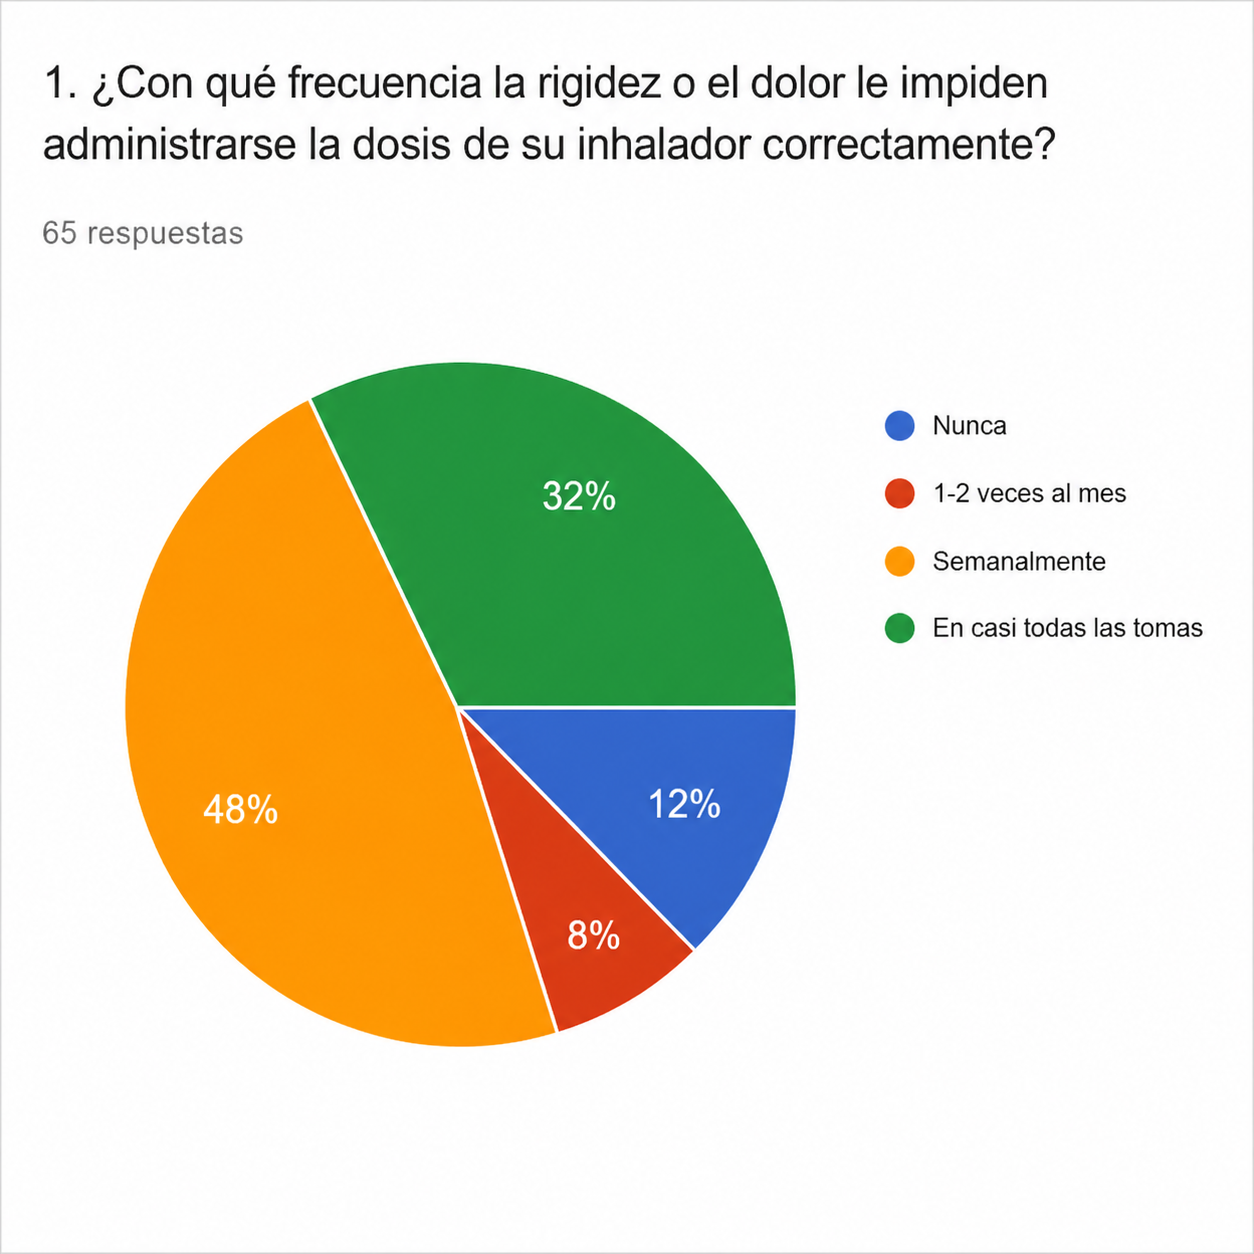
\includegraphics[width=0.5\textwidth, trim=5bp 5bp 5bp 5bp, clip]{grafico1.png}
    \caption{Frecuencia de impedimento por rigidez o dolor.}
    \label{fig:grafico1}
    \end{figure}
    
    \item \textbf{2. ¿Qué característica considera más importante en un accesorio ergonómico para inhaladores?} \\
    Una abrumadora mayoría del 65\,\% señala \textit{Que reduzca el esfuerzo} como el factor clave. Un 22\,\% prioriza \textit{Que sea fácil de colocar}. El diseño debe centrarse en maximizar la ventaja mecánica por encima de cualquier otro factor secundario.

    \begin{figure}[H]
    \centering
    % Cambia los valores de trim a tu gusto (ej. 5bp = 5 puntos base)
    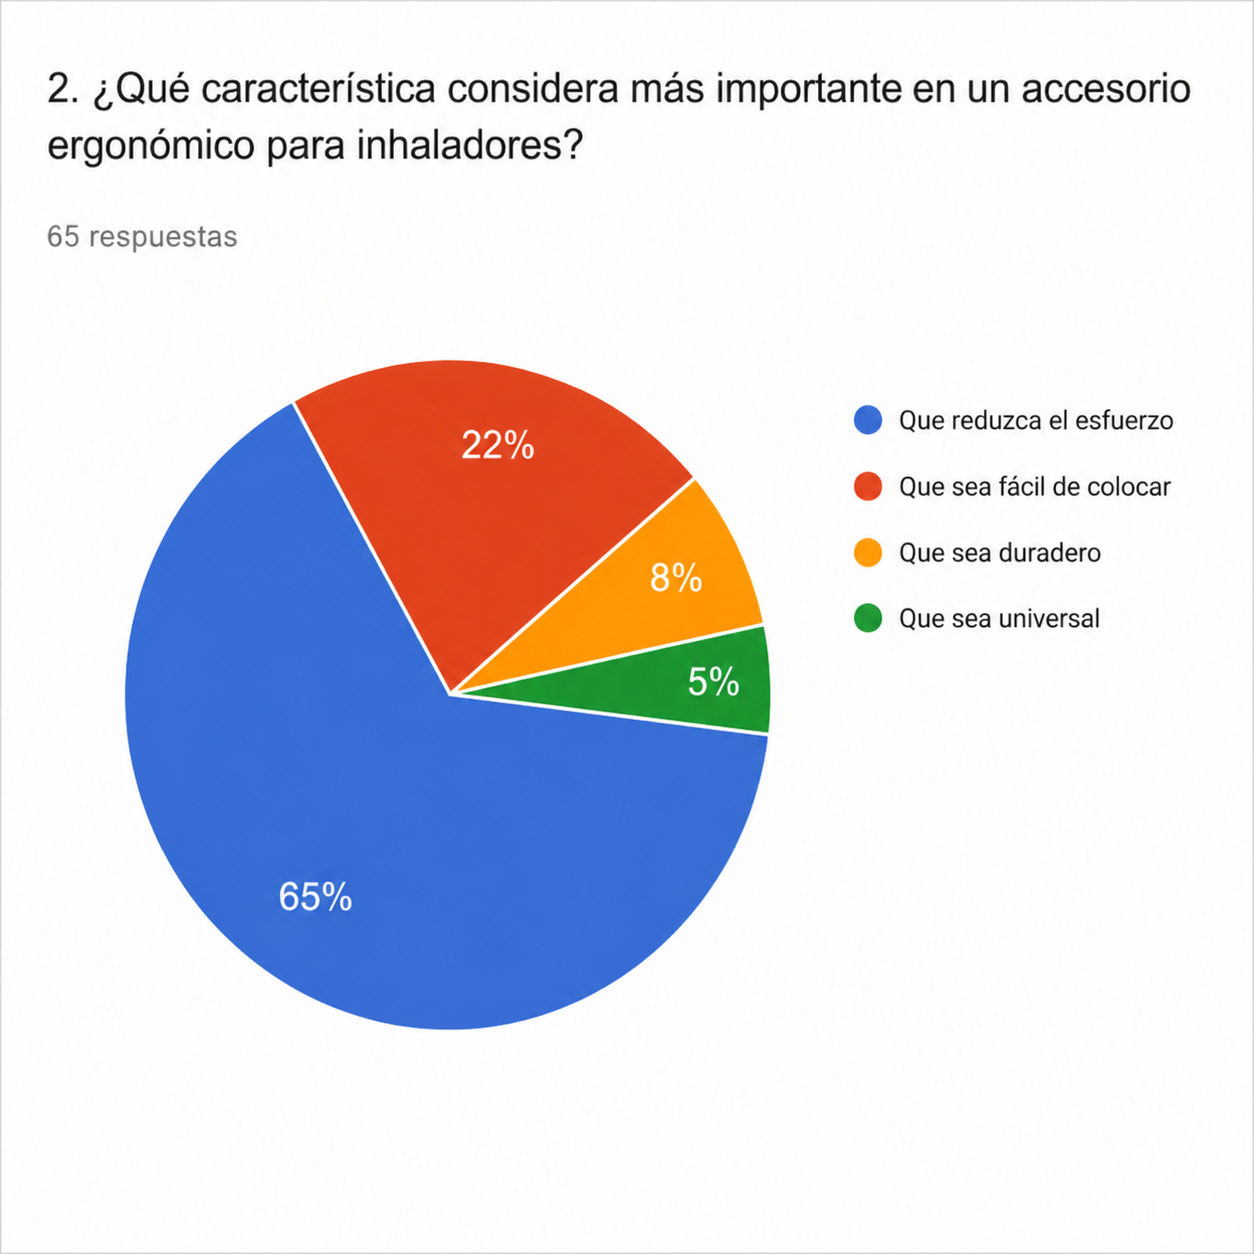
\includegraphics[width=0.5\textwidth, trim=5bp 5bp 5bp 5bp, clip]{grafico2.png}
    \caption{Prioridad de características.}
    \label{fig:grafico2}
    \end{figure}
    
    \item \textbf{3. ¿Qué tipo de superficie preferiría para la zona de agarre del adaptador?} \\
    El 58\,\% prefiere una zona de contacto \textit{Rugosa/antideslizante}, mientras que un 30\,\% opta por un acabado \textit{Blando}. Este resultado determina la necesidad de texturizar la zona de empuje palmar en los futuros moldes de inyección para asegurar la fricción.

    \begin{figure}[H]
    \centering
    % Cambia los valores de trim a tu gusto (ej. 5bp = 5 puntos base)
    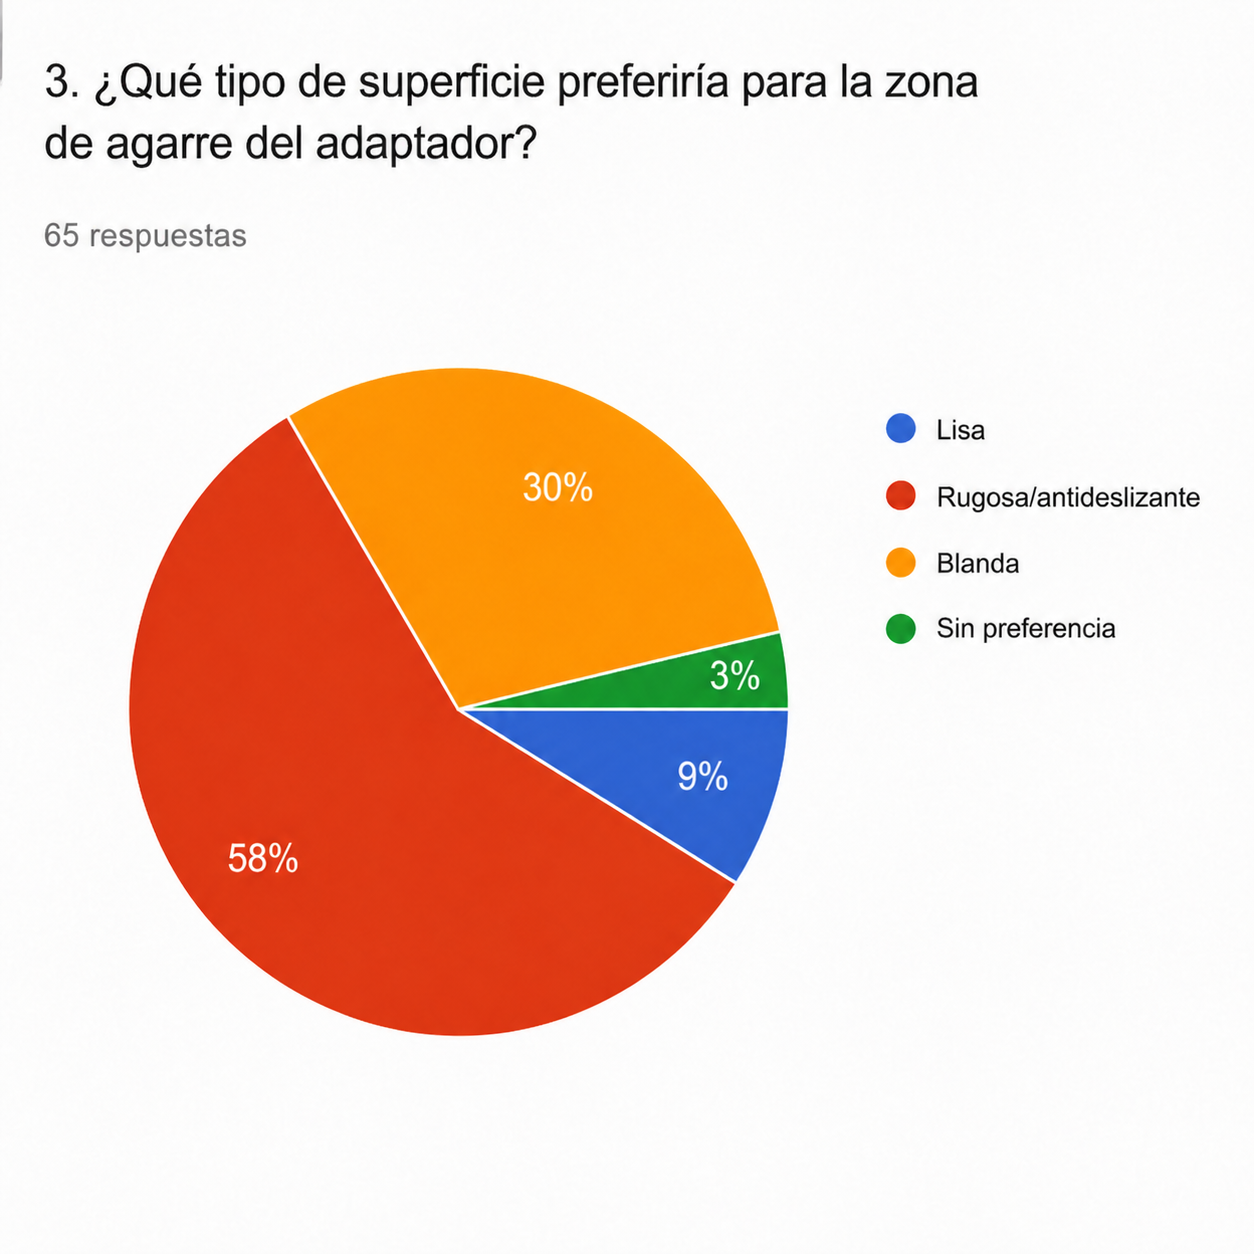
\includegraphics[width=0.5\textwidth, trim=5bp 5bp 5bp 5bp, clip]{grafico3.png}
    \caption{Preferencia de superficie y textura de agarre.}
    \label{fig:grafico3}
    \end{figure}
    
    \item \textbf{4. ¿Qué incremento de volumen aceptaría en su inhalador para ganar comodidad?} \\
    El 62\,\% de la muestra acepta un \textit{Aumento medio para llevar en bolso}. Un 25\,\% toleraría un tamaño \textit{Grande y exclusivo para uso doméstico}. La portabilidad de bolsillo estricta queda descartada, y esto otorga mayor libertad dimensional para diseñar el brazo de palanca.

    \begin{figure}[H]
    \centering
    % Cambia los valores de trim a tu gusto (ej. 5bp = 5 puntos base)
    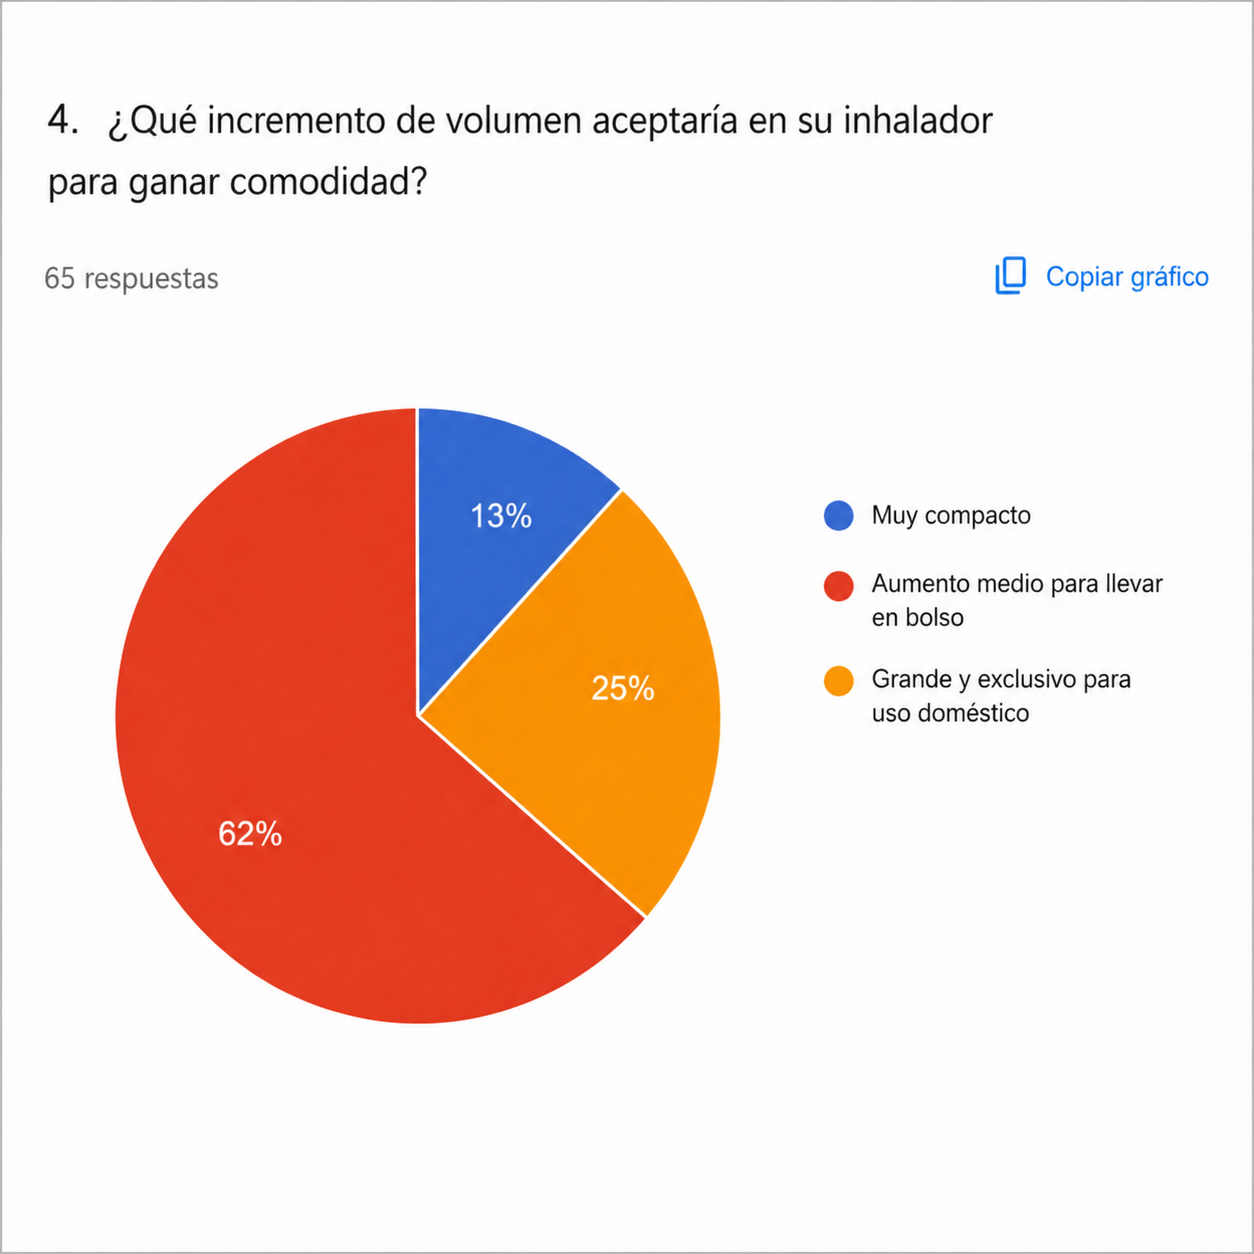
\includegraphics[width=0.5\textwidth, trim=5bp 5bp 5bp 5bp, clip]{grafico4.png}
    \caption{Tolerancia al volumen del dispositivo.}
    \label{fig:grafico4}
    \end{figure}
    
    \item \textbf{5. ¿Qué presupuesto máximo consideraría aceptable para este adaptador reutilizable?} \\
    El 54\,\% considera adecuado un precio de venta \textit{Entre 10€ y 20€}. Un 30\,\% preferiría un coste de \textit{Menos de 10€}. Este margen económico obliga a optimizar la cantidad de piezas y simplificar el proceso de ensamblaje industrial.

    \begin{figure}[H]
    \centering
    % Cambia los valores de trim a tu gusto (ej. 5bp = 5 puntos base)
    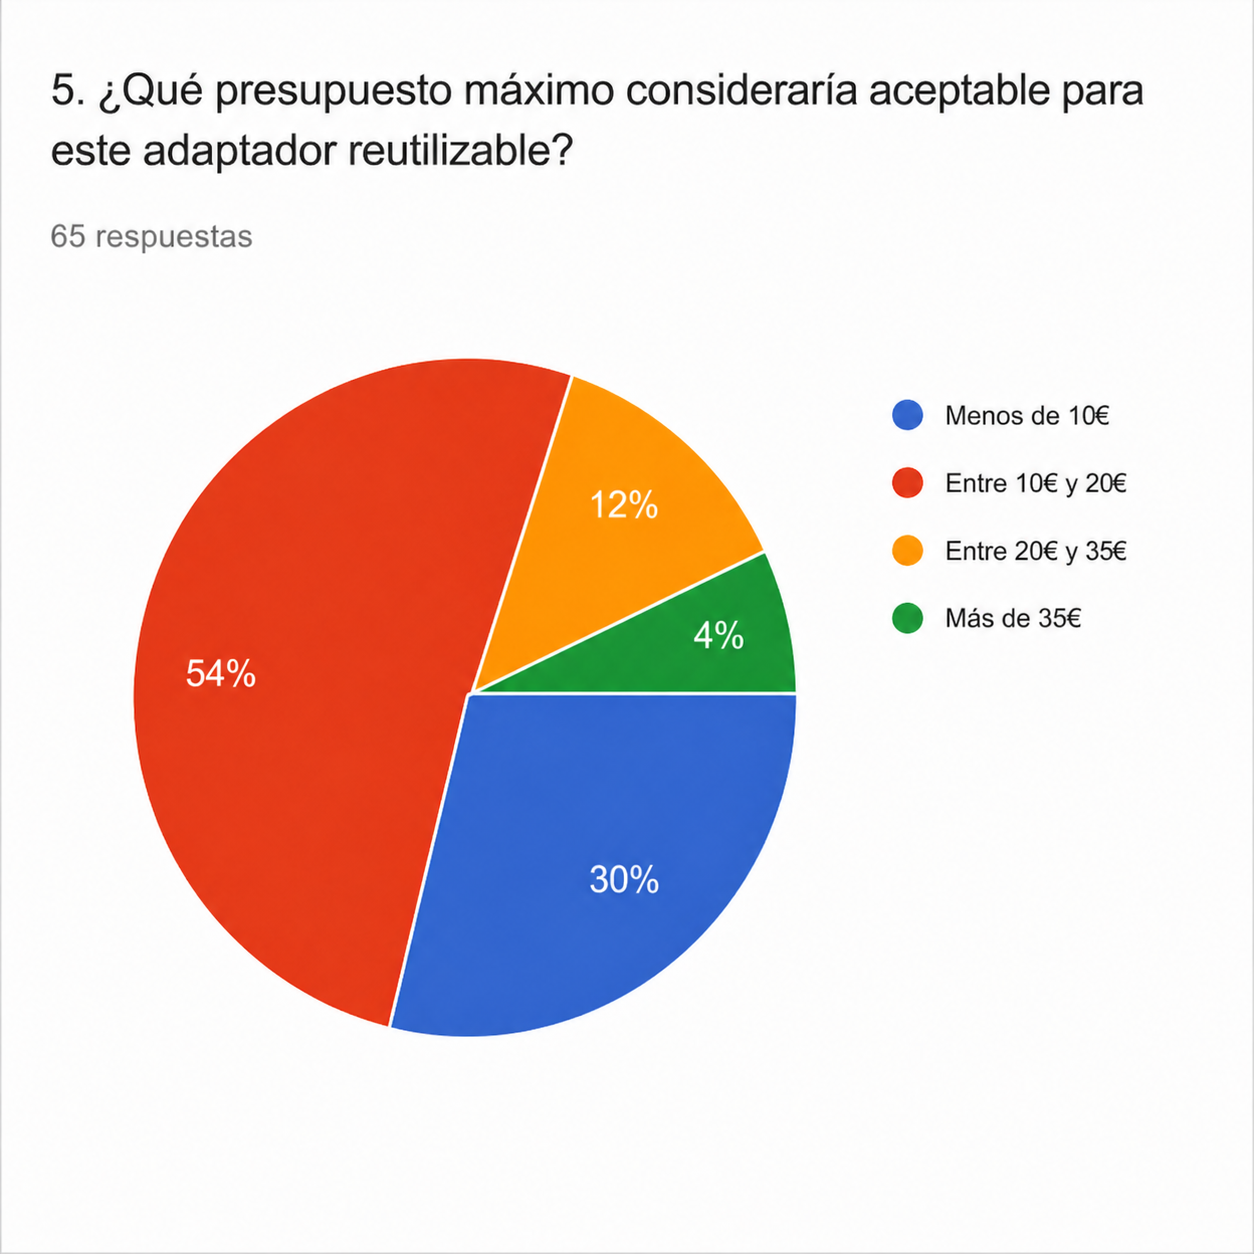
\includegraphics[width=0.5\textwidth, trim=5bp 5bp 5bp 5bp, clip]{grafico5.png}
    \caption{Disposición a pagar por el adaptador.}
    \label{fig:grafico5}
    \end{figure}
\end{itemize}

\section{JUSTIFICACIÓN DE LAS DECISIONES}
Las preguntas han sido seleccionadas para cubrir los bloques de \textbf{Ergonomía, fabricación y mercado}. Los datos extraídos de la entrevista validan la necesidad de desarrollar una solución basada en el principio de la palanca. Las declaraciones de la usuaria confirman que el diseño debe sustituir el movimiento de pinza dactilar por un empuje palmar. Además, la tolerancia al aumento de volumen permite al equipo priorizar la ergonomía estructural sobre la miniaturización del dispositivo.

\vspace{1.5cm}

 \vspace{0.5cm}
    \noindent\begin{minipage}{\textwidth}
    \begin{flushright}
        En Málaga, a \today
    \end{flushright}
    \vspace{2cm}

    \noindent
    \begin{minipage}[t]{0.45\textwidth}
        \centering
        \rule{6cm}{0.6pt} \\
        \textbf{Fdo. D. Sergio Carmona Muñoz} \\
        Colegiado Nº 06424 \\
        DNI: 26291930D
    \end{minipage}
    \hfill
    \begin{minipage}[t]{0.45\textwidth}
        \centering
        \rule{6cm}{0.6pt} \\
        \textbf{Fdo. D. Juan Gabriel Navarro Valdivielso} \\
        Colegiado Nº 06425 \\
        DNI: 77666662D
    \end{minipage}

    \vspace{2cm}

    \noindent
    \begin{minipage}[t]{0.45\textwidth}
        \centering
        \rule{6cm}{0.6pt} \\
        \textbf{Fdo. D. Antonio Sánchez Doña} \\
        Colegiado Nº 06423 \\
        DNI: 79380534J
    \end{minipage}
    \hfill
    \begin{minipage}[t]{0.45\textwidth}
        \centering
        \rule{6cm}{0.6pt} \\
        \textbf{Fdo. D. Iván de la Torre Segato} \\
        Colegiado Nº 06421 \\
        DNI: 79383630G
    \end{minipage}
\end{minipage}
    \vspace{1cm}

    % ======================================================
% HOJA EN BLANCO CON MARCA DE AGUA
% ======================================================
\newpage
\pagestyle{fancy}

\begin{tikzpicture}[remember picture, overlay]
    \node[opacity=0.1] at (current page.center) {
\includegraphics[width=12cm]{logo_definitivo.png}};
\end{tikzpicture}

% Empujamos el texto hacia la parte inferior del folio
\vspace*{8.5cm} 
\begin{center}
    \textit{Esta hoja ha sido dejada deliberadamente en blanco.}
\end{center}
\vfill


\end{document}

